% ****** Start of file apssamp.tex ******
%
%   This file is part of the APS files in the REVTeX 4.1 distribution.
%   Version 4.1r of REVTeX, August 2010
%
%   Copyright (c) 2009, 2010 The American Physical Society.
%
%   See the REVTeX 4 README file for restrictions and more information.
%
% TeX'ing this file requires that you have AMS-LaTeX 2.0 installed
% as well as the rest of the prerequisites for REVTeX 4.1
%
% See the REVTeX 4 README file
% It also requires running BibTeX. The commands are as follows:
%
%  1)  latex apssamp.tex
%  2)  bibtex apssamp
%  3)  latex apssamp.tex
%  4)  latex apssamp.tex
%%
\documentclass[%
 reprint,
%superscriptaddress,
%groupedaddress,
%unsortedaddress,
%runinaddress,
%frontmatterverbose,
%preprint,
%showpacs,preprintnumbers,
%nofootinbib,
%nobibnotes,
%bibnotes,
 amsmath,amssymb,
 aps,
%pra,
%prb,
%rmp,
%prstab,
%prstper,
%floatfix,
]{revtex4-1}


\usepackage{graphicx}% Include figure files
\usepackage{dcolumn}% Align table columns on decimal point
\usepackage{bm}% bold math
\usepackage{hyperref}% add hypertext capabilities
%\usepackage[mathlines]{lineno}% Enable numbering of text and display math
%\linenumbers\relax % Commence numbering lines

%\usepackage[showframe,%Uncomment any one of the following lines to test
%%scale=0.7, marginratio={1:1, 2:3}, ignoreall,% default settings
%%text={7in,10in},centering,
%%margin=1.5in,
%%total={6.5in,8.75in}, top=1.2in, left=0.9in, includefoot,
%%height=10in,a5paper,hmargin={3cm,0.8in},
%]{geometry}
%

\usepackage{xcolor}
\newcommand{\DP}[1]{\noindent \color{cyan} (DP: #1)\normalcolor}
\newcommand{\AZ}[1]{\noindent \color{purple} (AZ: #1)\normalcolor}
\newcommand{\add}[1]{\noindent \color{blue} #1 \normalcolor}
\newcommand{\del}[1]{\noindent \color{red} \st{#1}\normalcolor}
\newcommand{\AM}[1]{\noindent \color{magenta} (AA: #1)\normalcolor}
\def\red{\textcolor{red}}
%
\begin{document}
%
\preprint{APS/123-QED}

\title{Temporal Evolution of flow in Pore-Networks:\\ From Homogenization to Instability} 
% Force line breaks with \\
% \thanks{A footnote to the article title}%

\author{Ahmad Zareei}
\affiliation{School of Engineering and Applied Sciences, Harvard University, Cambridge, MA, 02148}%\altaffiliation[]{SEAS, Pierce Hall}%Lines break automatically or can be forced with \\
\author{Deng Pan}%
\affiliation{School of Engineering and Applied Sciences, Harvard University, Cambridge, MA, 02148}%\altaffiliation[]{SEAS, Pierce Hall}%Lines break automatically or can be forced with
\author{Ariel Amir}%
\email{arielamir@seas.harvard.edu}
\affiliation{School of Engineering and Applied Sciences, Harvard University, Cambridge, MA, 02148}%\altaffiliation[]{SEAS, Pierce Hall}%Lines break  automatically or can be forced with
% need to figure out how to reference dagger

% \author{}
% \altaffiliation[]{SEAS, Pierce Hall}%Lines break automatically or can be forced with \\
% \author{}%
%  \email{}
% \affiliation{% SEAS, Pierce Hall, Harvard University}%

% \collaboration{MUSO Collaboration}%\noaffiliation

\date{\today}% It is always \today, today,
             %  but any date may be explicitly specified

\begin{abstract}
We study the dynamics of flow-networks in porous media using a pore-network model. First, we consider a class of erosion dynamics assuming a constitutive law depending on flow rate, local velocities, or shear stress at the walls. We show that depending on the erosion law, the flow may become uniform and homogenize, stay as it is, or become unstable and develop channels. By defining an order parameter capturing different behaviors we show that a phase transition occurs depending on the erosion dynamics. Using a simple model, we identify quantitative criteria to distinguish these regimes. Lastly, we show that pores clogging at the initial stages show analogous behaviors depending on clogging dynamics. % , however, due to the pore throat blockages and changes in the network connections the evolution diverges from its initial trend.

% \begin{description}
% \item[Usage] Secondary publications and information retrieval purposes.
% \item[PACS numbers] May be entered using the \verb+\pacs{#1}+ command.
% \item[Structure] You may use the \texttt{description} environment to structure your abstract; use the optional argument of the \verb+\item+ command to give the category of each item.
% \end{description}
\end{abstract}

% \pacs{Valid PACS appear here}% PACS, the Physics and Astronomy
                             % Classification Scheme.
%\keywords{Suggested keywords}%Use showkeys class option if keyword
                              %display desired
\maketitle
%%%%%%%%%%%%%%%%%%%%%%%%%%%%%%%%%%%%%%%%%%
%%%%%%%%% \tableofcontents %%%%%%%%%%%%%%%
%%%%%%%%%%%%%%%%%%%%%%%%%%%%%%%%%%%%%%%%%%
%%%%%%%%%% \section{Introduction} 
%%%%%%%%%%%%%%%%%%%%%%%%%%%%%%%%%%%%%%%%%%
%%%%% The fluids %%%%%%%%%%%%%%%%%%%%%%%%%
%%%%%%%%%%%%%%%%%%%%%%%%%%%%%%%%%%%%%%%%%%

Fluid flow through a porous medium undergoing a dynamical change in its network of micro-structure is a challenging problem and has many environmental and industrial applications~\cite{fraggedakis2015flow,sahimi2011flow,schlesinger1999carbon,herzig1970flow,tien1979advances,jaisi2008transport,carrel2018biofilms,seymour2004anomalous,duduta2011semi,sun2019hierarchical,marbach2016pruning,tero2010rules,alim2013random,heaton2010growth}.
% , such as oil recovery~\cite{fraggedakis2015flow,sahimi2011flow}, CO$_2$ sequestration~\cite{schlesinger1999carbon}, water filtration/separation~\cite{herzig1970flow,tien1979advances,jaisi2008transport,carrel2018biofilms,seymour2004anomalous}, energy storage~\cite{duduta2011semi,sun2019hierarchical}, or biological applications \cite{marbach2016pruning,tero2010rules,alim2013random,heaton2010growth}. 
The disordered pore structure of a porous medium results in a heterogeneously distributed fluid flow between the pores.
% Fluid flow in a porous medium is often heterogeneously distributed between the pores as a result of a highly disordered pore structure.
Due to the fluid flow, the pore structure can further change dynamically either through the erosion of pore boundary walls or deposition/sedimentation of material on the boundary of the pores. Such heterogeneous and dynamical changes of the solid structure affect the pore-level fluid flow which in turn affects the dynamical changes to the pore structure. This feedback mechanism along with the initial heterogeneous fluid flow complicates the dynamical process and makes it difficult to understand and predict the porous media behavior. Nonetheless, an understanding of the dynamical change is essential to improve any of the porous media applications where the pore network changes over time, applications such as groundwater remediation and precipitation of minerals in rocks~\cite{rad2013pore}, biofilm growth in water filtration, and protective filters \cite{herzig1970flow,tien1979advances,jaisi2008transport,carrel2018biofilms,seymour2004anomalous}, as well as enhanced oil recovery with polymer flooding \cite{lake2014fundamentals,parsa2020origin}, or water-driven erosion \cite{schorghofer2004spontaneous,mahadevan2012flow}. 

% to the pore structure affects local fluid flow as well as bulk properties of the medium. 
% Understanding flow behavior is important to improve any of the the applications where the pore structure changes dynamically either by erosion of the boundary wall or deposition/sedimentation of material on the boundary. Changes in the micro-structure and solid boundaries affect local fluid flow as well as the bulk properties. The  erosion or deposition process in a porous media plays an essential role in many environmental and industrial applications such as groundwater remediation and precipitation of minerals in rocks, bio-film growth in water filtration and the design of protective filters,  as well as enhanced oil recovery with polymer flooding, water-driven erosion. The structures of such porous media are usually highly disordered with a heterogeneous distribution of pore-level flow velocities. 
%% 

% Albeit there is an abundance of applications in understanding 
% Despite the importance of understanding flow evolution in porous structures exposed to erosion and deposition,it 
% \footnote{It can be shown that the rate of change in tube's radius in \cite{reddi2000permeability} assuming a dilute solution becomes proportional to local fluid velocity},


In light of the plethora of applications, it is surprising that the evolution of porous structures exposed to erosion and deposition has only been partially understood both theoretically and experimentally. In order to model erosion in porous materials, different models have been used where erosion is assumed to be locally proportional to different flow parameters. Some studies have focused on the erosion of the pore structure proportional to the shear stress at the walls \cite{jager2017channelization,ristroph2012sculpting,hacking1996shear,wan2004investigation}, or proportional to the power dissipated by the flow~\cite{steeb2007modeling,marot2012study,sibille2015internal}. 
More recently it has been shown that using a coarse-grained model with an erosion rate depending on the local pressure gradient, different branching instability can be reached in a porous material~\cite{derr2020flow,mahadevan2012flow}.  
Similarly, in clogging, deposition rate based on local fluid flux, velocity, or even at a constant rate independent of any flow parameters has been used~\cite{yang2017pore,reddi2000permeability,boccardo2014microscale}. In order to unify the different approaches, we use a general continuous model which allows us to study the effect of different erosion or clogging dynamics with a single constitutive law. Additionally, we use a network approach~\cite{alim2017local,fatt1956network, blunt2013pore,stoop2019disorder,bryant1993network} to study the flow dynamics in the porous media.  The network approach has the advantage of not requiring coarse-grained homogenization and is computationally simple allowing us to simulate larger domains.

% (which is the same as shear at the walls),
% to capture the flow dynamics

% Despite all of the different models, a consensus on the dynamics of erosion or clogging is missing.\red{focus more on the network model} The adventage versatile law network approach -> does not need homogenization or meanfield assumption


% Since the dynamics of erosion in a porous material is not well understood, 

% A phenomenological discrete network-based model~\cite{alim2017local,fatt1956network, blunt2013pore,stoop2019disorder,bryant1993network} is used to model the hydrodynamically driven erosion or clogging in a porous material.
% In the network model, the pores are represented by spherical nodes connected with edges represented by cylindrical tubes. 

The network of pores inside the solid structure is connected together through pore-throats that effectively show resistance to the fluid flow between the pores (Fig.~\ref{fig:fig1}a). In a network model, the pores/voids of the porous medium are represented by a two- or three-dimensional lattice of nodes. The edges between the nodes of the network represent the pore-throats between the pores and are modeled using cylindrical tubes characterized by their radius and length. 
Network-based models have successfully shown to capture key properties of fluid flow in a porous material such as the probability distribution of fluid flux~\cite{alim2017local}, the permeability scaling during clogging~\cite{shima2021}, or the first fluidized path in a porous structure~\cite{fraggedakis_chaparian_tammisola_2021}. 
% Using such network models, it has been shown that the probability distribution of fluid flux in a porous material is universal when the porous material is random enough. Furthermore, during the clogging process, the usage of Kozeny-Carman fails to correctly predict the porosity since all the length scales are not eroding at the same time (the erosion only happens at the corss sections and not along the length of a porous material). New relation based on the variation in porosity has been proposed that can successfully find the relation between porosity and permeability variation using such models which is verified experimentally.
The degradation of the solid skeleton (i.e., erosion) or deposition of material on the pore throats (i.e., clogging) in such networks is modeled by the change (increase or decrease) in the radius of the edges connecting the pores which ultimately translates in the changes in the flow resistance between the pores. Using a general local erosion law that can model different dynamics, we show a variety of behaviors are possible. The network can either move toward stability and homogenization, stay as it is with no significant change in network statistics, or become unstable and develop channels. Using numerical solutions with an erosion model on a random network we show the emergence of two behaviors and morphologies are possible through selective erosion and subsequent flow enhancement. Using a simplified model we capture the underlying physics and furthermore show a phase transition occurs depending on the parameters of the model. 
% Here, based on the porous network model, we link various erosion laws with different large-scale behaviors and show a variety of behaviors that can be observe
% In order to better understand the effect of different erosion dynamics in a porous based on local parameters, 
% network model has been successful in predicting the first open channeel \cite{fraggedakis_chaparian_tammisola_2021} and capturing the fluid flow distribution \cite{alim2017local}
% \cite{fatt1956network} 
% \cite{blunt2013pore}
% \cite{stoop2019disorder}
% Consequently, clogging effects are excluded from these assumptions. Thus, the eroded fines can be transported through the porous material within these statistically homogeneous distributed channels
% Albeit there is an abundance of applications, the evolution of structures exposed to erosion and deposition is in general not easily predictable and usually requires the use of numerical techniques.
% However, this process is difficult to model due to diverse processes that may arise, including particle advection through the pore space by fluid flow, adsorption and deposition onto the solid matrix, and erosion or resuspension.
% \begin{itemize}
% \item Importance of porous media
% \item importance of dynamics in porous media
% \item we study evolution with a network model
% \end{itemize}

%%%%%%%%%%%%%%%%%%%%%%%%%%%%%%%%%%%%%%%%%%%5
% \section{Methods \& Results}
%%%%%%%%%%%%%%%%%%%%%%%%%%%%%%%%%%%%%%%%%%%%5
\begin{figure}[h]
    % \centering
    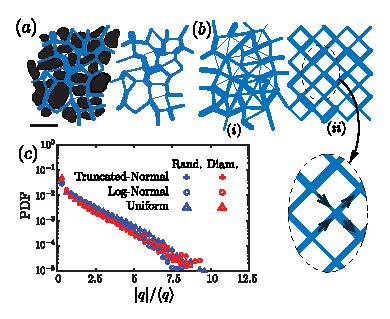
\includegraphics[width = 0.45\textwidth]{Figs/Fig1_pppp.eps}
    \caption{(a) Cross section of a porous media obtained using  computerized tomography (CT) scan of a sandstone sample (CT image taken from \cite{akanji2010finite}). The scale in the bottom left shows $1$mm. The network of pores and throats is highlighted in blue. In the network model, the pores are represented with nodes and the throats between pores are approximated with tubes connecting the pores together. (b) Schematic of a topologically random network (i); and a structured diamond grid network (ii). The edge diameters in both networks are randomly distributed. The inset figure shows the conservation of mass at each node. (c) The universal probability distribution function (PDF) of fluid flux for a topologically random (in blue) or diamond network (red) with a highly disordered random net including uniform (triangles), log-normal (circles), and truncated normal (plus) distributions. The distribution parameters are chosen such that the coefficient of variation (the ratio of the standard deviation to the mean) becomes $0.5$ which results in a highly disordered pore throat distribution. Generally, in a highly disordered random network, the PDF of normalized fluid flux becomes independent of the network and follows a universal distribution with an exponential tail. }\label{fig:fig1}
\end{figure}
%
% \AZ{Things are not topoligically random }
% \AZ{random end }
% \AZ{structured allows for mean field theory}
% \AZ{the edges are the same - exponential where it is coming from}
% \AZ{boundary between phases, where the mean fields hold}

  % Flow through pores and throats of a porous medium can be modeled using a pore network model \cite{alim2017local,fatt1956network, blunt2013pore,stoop2019disorder}. In a network model, the pores/voids of porous medium are represented by a two- or three-dimensional lattice of nodes. The edges between the nodes of the network represent the pore-throat between the pores and are modeled using cylindrical tubes characterized by their radius and length (see Fig. \ref{fig:fig1}(a)). The pore-network model is well suited for the simulation of low-Reynolds fluid flow and has proved to capture the flow dynamics of porous media \cite{alim2017local} and also the first fluidized path \cite{fraggedakis_chaparian_tammisola_2021}. We use a structured/unstructured network with randomly distributed nodes and edge length. 
% It has been shown that flow through such network correctly captures the exponential tail for distribution of fluid velocities through a porous medium. 


\textit{Methods and Results}-- We consider low-Reynolds fluid flow through the porous network, i.e.,  $\rho u r/\mu \ll 1$ where $\rho$ is the fluid density and $\mu$ is the kinematic viscosity, $u$ and $r$ are characteristic fluid velocity and pore radius. In such conditions, the fluid flow in each tube follows the Poiseuille law
 $ p_i - p_j  = ({8 \mu l_{ij}}/{\pi r_{ij}^4}) q_{ij}$ where $p_i,p_j$ represents pressures at neighboring nodes $i$, $j$, and $r_{ij}, l_{ij}, q_{ij}$ are respectively the radius, length, and fluid flow rate at the edge connecting pores $i$ and $j$. The coefficient ${\pi r_{ij}^4}/{8 \mu l_{ij}}$ which relates the fluid flux to the pressure difference can be considered as the conductance $C_{ij}$ of the edge $ij$ in the pore-network. In addition to Poiseuille flow at the edges,  the total incoming flow at a node should be equal to the total outgoing flow in order to conserve mass. The conservation of mass at pore $i$ can be written as $\sum_{j\in \mathcal{N}(i)} q_{ij} =0$ where $\mathcal{N}(i)$ represents all the neighboring nodes of node $i$. First, we consider a topologically random network of nodes constructed using a uniform distribution of $N_x\times N_y$ nodes in a planar domain $\left[0,L_x\right]\times \left[0,L_y\right]$ where the nodes connectivity are obtained using Delaunay triangulation (see Fig. \ref{fig:fig1}b(i) for a part of such network). The radius of the edges is considered as independent and identically distributed random variables sampled from a probability distribution that can be either uniform, log-normal, or a truncated normal distribution (see supplementary material S1 for more details).  Assuming a pressure difference between the boundary nodes at the left and the right boundary, the pressure at the nodes, and the fluid flow rate at the tubes can be obtained by solving the corresponding set of linear equations. We find that for large enough randomness in the edge radii (i.e., $\text{std}(r_{ij})/\text{mean}(r_{ij})\geq 0.5$), the PDF is well described by a single exponential distribution as shown in Fig. \ref{fig:fig1}c. The exponential form of the PDF reflects the relatively small number of edges with extremely large fluid fluxes. The exponential distribution of fluid flux obtained here is similar to the earlier experimental or numerical measurements~\cite{datta2013spatial,shima2021,alim2017local}.  Next, we consider a structured diamond-grid of pores (Fig. \ref{fig:fig1}b(ii)) which significantly simplifies the geometrical complexity of the network. First, we find that the PDF of normalized fluid flux remains unchanged in such networks for various distributions and in fact matches with an unstructured random network (Fig. \ref{fig:fig1}c). The diamond grid allows us to analytically track the propagation of fluid into the network and calculate the distribution of fluid flux using a mean-field approximation (see supplementary material S3). Using a similar idea proposed for the force distribution in granular materials~\cite{liu1995force,coppersmith1996model,alim2017local}, it can be shown that the PDF of normalized fluid flux inside a highly disordered porous material converges to a universal distribution with an exponential form, i.e., $p(\hat{q}) \propto e^{-\alpha \hat{q}}$ for large $\hat{q}$ where $\hat{q}$ is the normalized fluid flux $\hat{q} = {q}/\langle q \rangle$ (see supplementary materials S3). This result indicates that the diamond grid network of pores where cylindrical edges between the pores have a highly disordered distribution is sufficient to capture the statistics of a heterogeneous fluid flow inside a porous material. 
 
 % In the following parts we show the results of a diamond grid, and the results for a random-graph is presented in the supplementary material.  
 
%  independent of the pore structure, becomes exponentially distributed. 
%  Considering a random \AZ{needs explicit definition} or structured network with a random distribution of tube's radius/length (i.e., effectively their flow resistance) and a 
%  For a large enough randomness in the edge resistances between the pores $R_{ij}$, the probability distribution of flux in the tubes normalized by the average flux follows a universal curve with an exponential tail, i.e., $P(\hat{q}) \propto e^{-\alpha \hat{q}}$ for large $\hat{q}$ where $\hat{q}$ is the normalized fluid flux $\hat{q} = {q}/\langle q \rangle$ (See Fig. \ref{fig:fig1}c and supplementary material for more details). This PDF of fluid flux $q$ has been shown to correctly captures the exponential tail for the fluid flux in a porous medium \cite{alim2017local,shima2021}.
%


% Note that the flux $q_ij$ depends on the pressure gradient between nodes i.e. $(p_i-p_j)/l_{ij}$. On the other hand 
% We first start with a numerical model, where we assume a network of $200\times 100$ tubes in the horizontal and vertical direction on a diamond lattice \AZ{better motivation: explain and discuss the meanfield picture behind figure 1c} (similar results for a general \AZ{needs definition} random network is presented in the supplemental materials). 
\begin{figure}[!h]
    % \centering
    \includegraphics[width = 0.48\textwidth]{Figs/Fig_2_Random_Network.png}
    \caption{Erosion in a network of pipes. The initial condition is shown with the label $t=0$ in the first row. Each row afterward corresponds to the simulation result after $N$ steps such that $\langle r_{t=N}\rangle=2r_0$ where $r_0 = \langle r_{t=0}\rangle$. The erosion law is based on Eq. \eqref{eq:erosion-law} where different powers of $n$ correspond to different models of erosion. The first column is a snapshot of the pore network, the second column is the PDF of normalized fluid flux $q/\langle q \rangle$, and the last column is the PDF of normalized radius $r/\langle r\rangle$.}\label{fig:fig2}
\end{figure}
%



In order to model erosion in porous media, we consider the abrasion in the throats which correspond to the change in the radius of the edges in the network. We model the dynamics of the change in the radius as 
%
\begin{align}
   \frac{dr_{ij}}{dt} = \alpha  \frac{|q_{ij}|^m}{r_{ij}^n} \label{eq:erosion-law}
\end{align}
%
\add{where $m,n,\alpha$ are constants. Different powers of $m$ and $n$ correspond to different physics in the erosion. Particularly, when $m=1$ and (i) $n=0$ the erosion depends on the amount of flux $q_{ij}$ passing through the edge; (ii) $n=2$ the erosion depends on the local velocities; (iii) $n=3$ the erosion depends on the shear force at the boundary of the throat.} \add{Additionally, $m=2$ and $n=6$ corresponds to the models considered in biological transport networks where the there the radius change has a quadratic dependence on wall shear stress~\cite{hu2013adaptation,ronellenfitsch2016global}.} We consider network of randomly distributed pores with  $N_x\times N_y$ pores in the horizontal and vertical directions. The randomly distributed points are connected using Delaunay triangulation. We initialize the network with a uniform random distribution of diameters within $[r_\text{min}, r_\text{max}]$ range with a large coefficient of variation such that  $\sigma_r/r_0\approx 0.5$ where $\sigma_r$ is the standard deviation, and $r_0 = \langle r \rangle$~\cite{alim2017local}. The flow inside the pores, PDF of flux in the tubes, and PDF of tube radii are shown in Fig. \ref{fig:fig2}. We assume a constant pressure difference between the left and the right boundaries. In each time step, we increase the local radius of the tubes based on the erosion law introduced in Eq. \eqref{eq:erosion-law}. Note that $r_{ij} (t+\delta t)  = r_{ij} (t)  + (\alpha \delta t)  q_{ij} (t)/ r^n_{ij} (t) $, where the coefficient $\alpha \delta t$ is chosen such that the maximum change in the radius at each time step is smaller than one-tenth  of the smallest tube's radius i.e. $\max (\Delta r_{ij}) \leq r_\text{min}/10$ of the smallest radius at the initial configuration.  This condition guarantees that at each step a small amount of material is eroded and there's no sudden change in the network. We further test the convergence by decreasing $\max(\Delta r_{ij})$ to half and we observe that the average relative change in the flux vector becomes $\aprrox 1.2\%$, and the PDFs remain intact without any change. We continue the simulations until $\langle r \rangle = 2 r_0$. 
%
The results of the simulations for different $n$ are shown in Fig. \ref{fig:fig2}. When $n=1$ or $2$,  the network develops channels. In such cases, the flow is dominated by a few edges carrying most of the flow while the rest of the network carries almost no flow. This can be seen in the PDF of the normalized radius which becomes bimodal. Furthermore, the PDF of the normalized fluid flux contains a small number of edges with very large flux values while the majority of the edges carry small flux. Contrary to $n=1,2$, when $n=3$ and the erosion depends on shear at the throats' boundary walls, we find that the flow patterns stay very close to the initial shape, however, with larger and exacerbated flux values. Although the maximum fluid flux increases, the PDF of normalized fluid fluxes remains almost exponential, and the PDF of diameters moves toward larger values. Increasing $n$ to larger values, $n=4$ or $5$, we find that the flow pattern in the network moves toward homogenization. Here, the tail of the normalized fluid flux distribution retracts and the distribution moves toward the average value. We further find that the PDF of the diameters moves toward the average and the coefficient of variation reduces. Running the simulations for longer times, we observe that the flow becomes completely uniform where only a single radius appears to carry the flow with the same fluid flux (i.e., the average value) for all the tubes in the network. In summary, we have observed a transition in the network behavior during erosion which happens at $n=3$: when $n<3$ the network moves toward developing channels, and when $n>3$ the erosion results in the homogenization of the flow.

\begin{figure}[!h]
    % \centering
    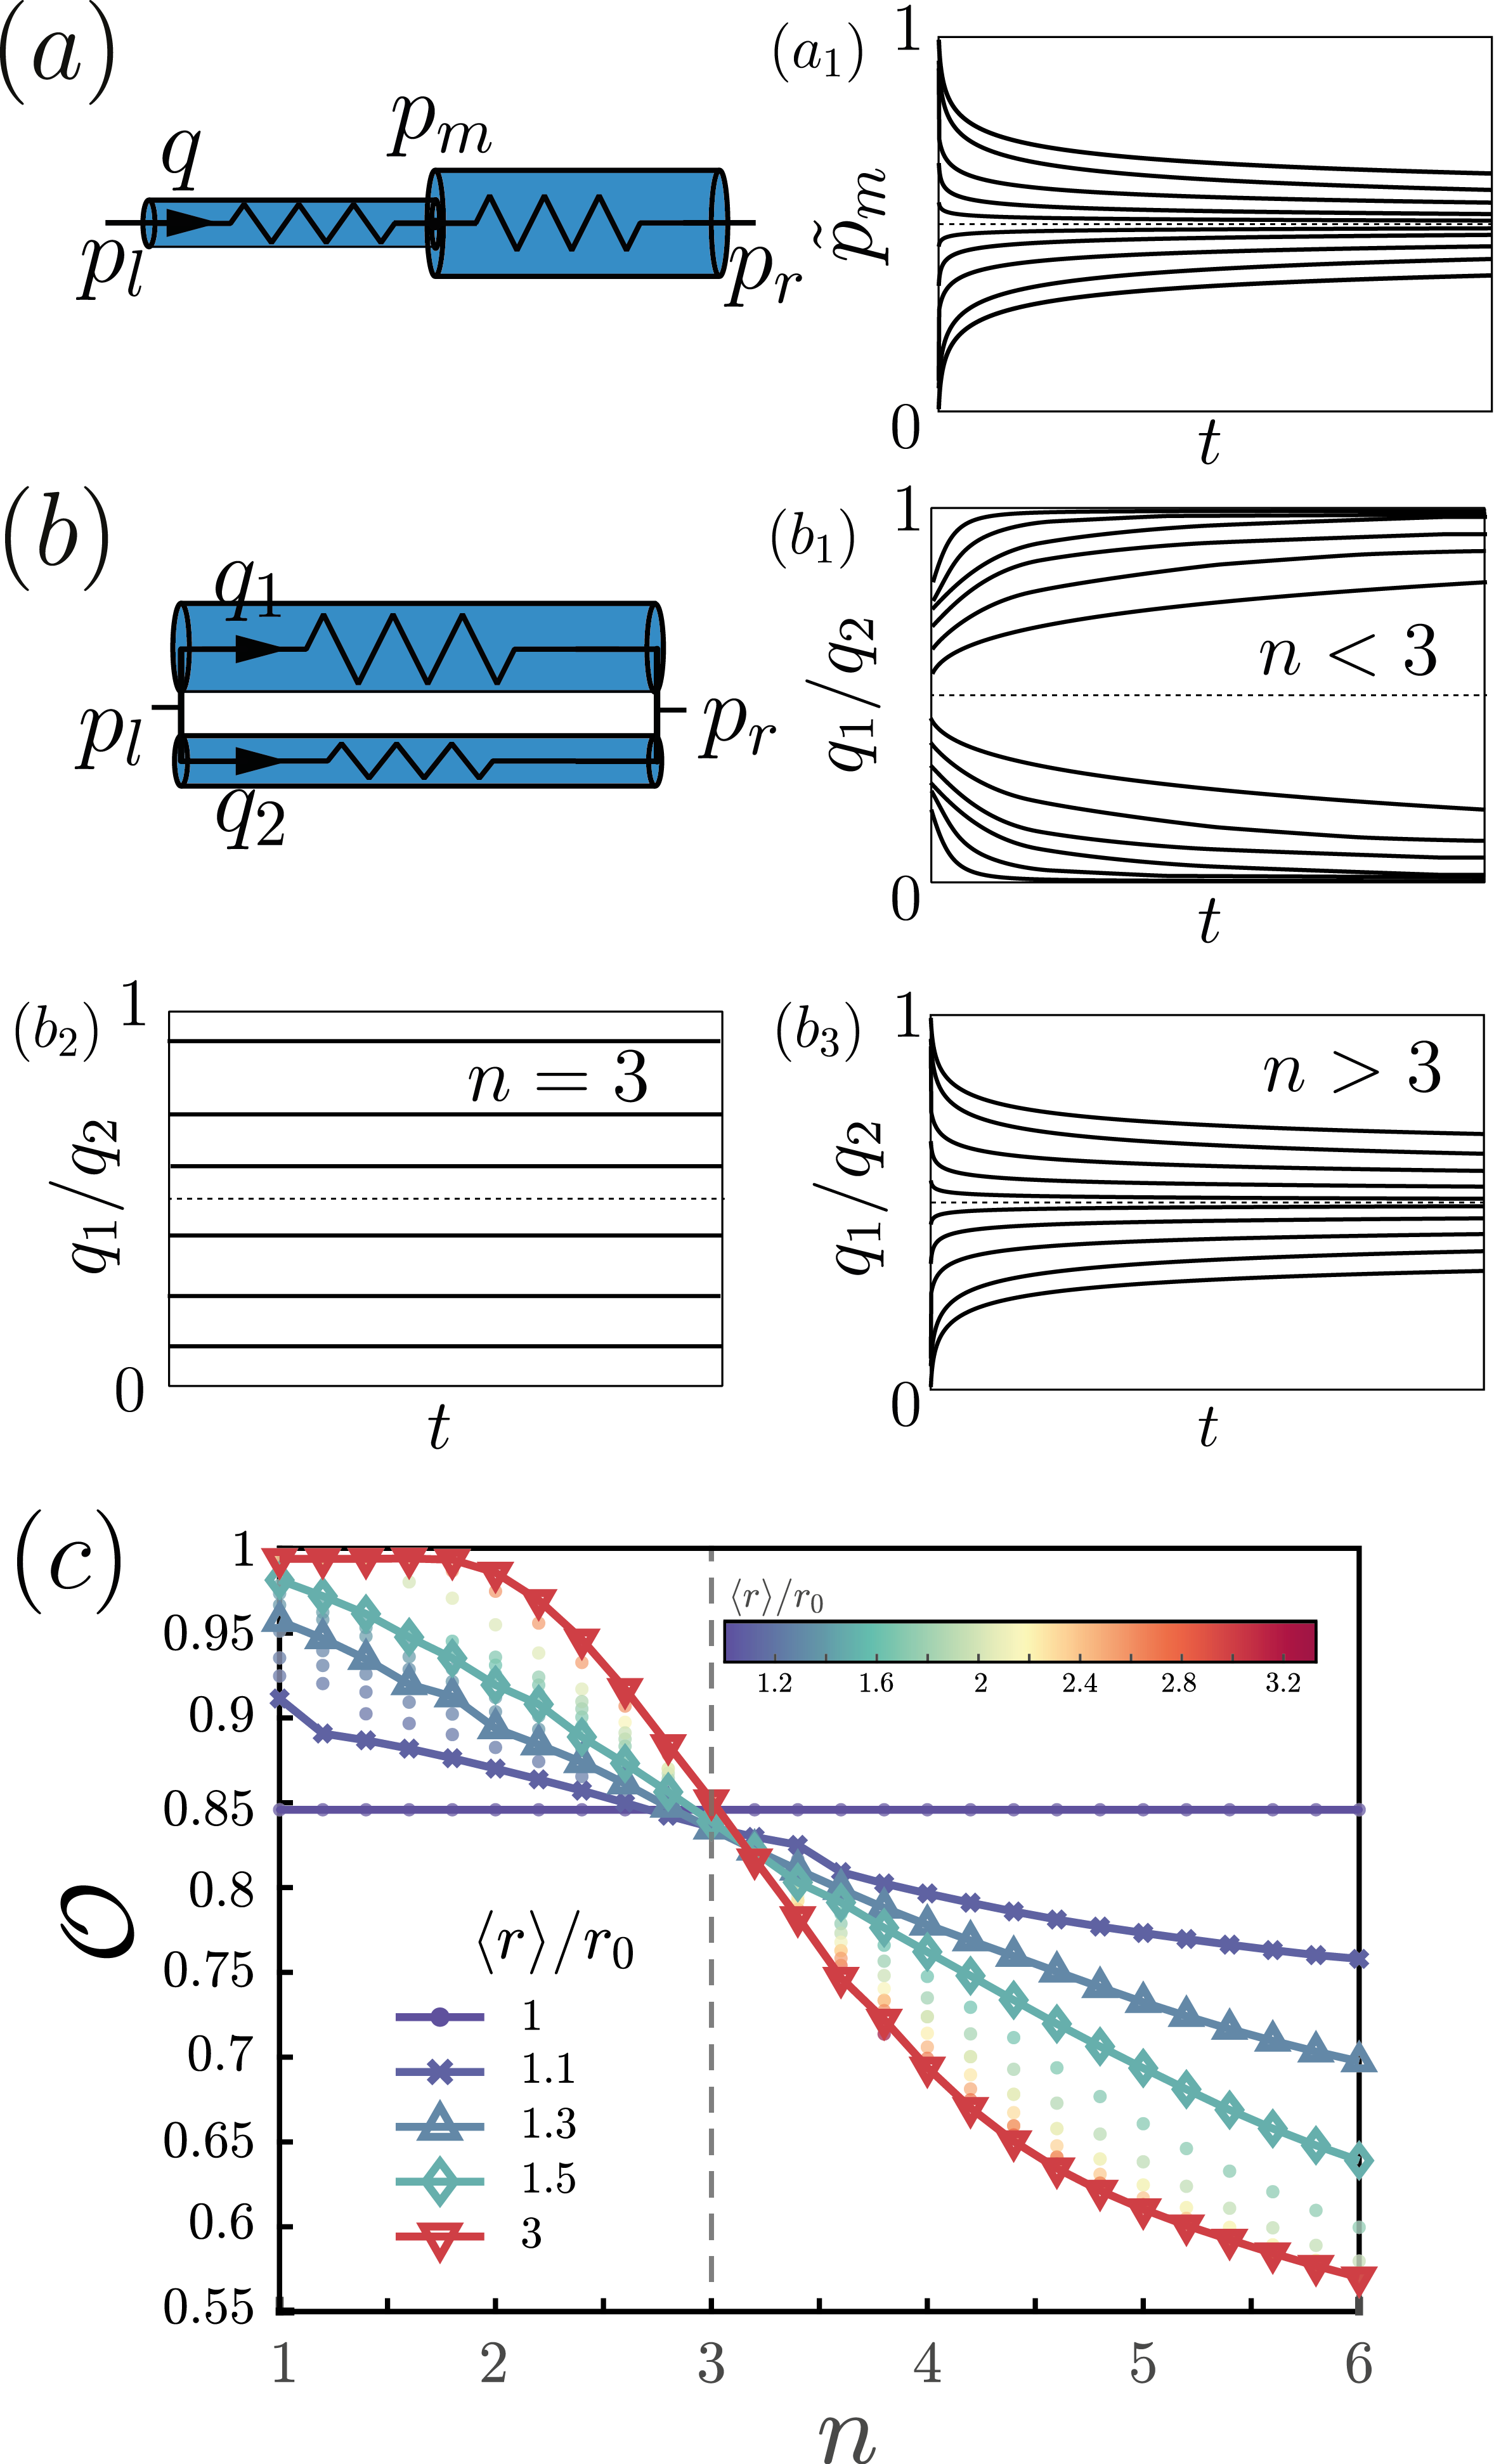
\includegraphics[width = 0.45\textwidth]{Figs/Fig3_new.png}
    \caption{Two tubes in (a) series  or (b) parallel configuration. When the tubes are in series configuration, the tubes have the same fluid flow rate $q$. The tube radius dynamically change with the erosion law $\dot{r_i}\propto q/r_i^n$. For any $n$, the normalized pressure at the junction between the tubes $\tilde p_m = (p_m - p_l)/(p_r-p_l)$ approaches $1/2$ which results in a homogenized pressure distribution  shown in (a$_2$). When the pipes are in parallel, however, the flow is distributed among the tubes based on their flow conductivity $C_1,C_2$. The local fluid flow rate then affects the erosion of the tub $\dot{r}_i\propto q_i/r_i^n$. When $n<3$ in the erosion law, the fluid flow eventually passes through a single tube, and channeling occurs; (b$_2$) when $n=3$, the flow ratio between the pipes does not change; and (b$_3$) when $n>3$ the flow ratio approaches $1/2$ which is the homogenization.(c) Order parameter $\mathcal{O}$ for different powers of $n$ plotted over time as the network structure is eroded and average edge radius is increasing $\langle r\rangle/r_0$. When $n<3$ the order parameter increases ($\mathcal{O}\to 1$) while the network is developing channels, and when $n>3$ the order parameter decreases ($\mathcal{O}\to 0$) while the network moves toward homogenization, and when $n=3$ the order parameter stays as it while the network statistics remains unchanged.}\label{fig:fig3}
\end{figure}



%%%%%%%%%%%%%%%%%%%%%%%%%%%%%%%%%%%%%%%%%
% \section{Simplified Model}
%%%%%%%%%%%%%%%%%%%%%%%%%%%%%%%%%%%%%%%%%%%5
%



\textit{Simplified Model}-- In order to understand the underlying reason behind the transition in network behavior during erosion for different powers of $n$, we focus on a simplified model with only two tubes in parallel or series (see Fig. \ref{fig:fig3}a,b). First, assuming two cylindrical tubes with radii $r_1,r_2$ in series and connected back to back, the flow is the same for the two tubes $ q_1 = q_2 = q$ (Fig. \ref{fig:fig3}a). The radius of each tube then changes with $dr_i/dt = \alpha q/r_i^n$ where $i=1,2$. Each tube can be considered as a resistor where its conductivity  $C_i =\pi r_i^4/8\mu l_i$ changes over time. In similarity with resistor networks, the pressure difference $\Delta P_i$ acts analogous to the voltage difference and the fluid flux $q_i$ is analogous to the current where we have $q_i = C_i \Delta P_i$. When the cylindrical tubes are in series, we find that the conductivity of each tube changes as $dC_i/dt \propto C_i^{(n-3)/4}$. As a result, each tube's conductivity increases with a rate depending on $n$, i.e. the larger the $n$ the faster it moves toward larger values. If we consider the pressure at the junction between tubes, we find that this middle point pressure moves toward the average value of pressure on both sides (see Fig. \ref{fig:fig3}(a$_1$)). As a result, when the tubes are in series, the erosion results in a homogenized distribution of pressure. Contrary to tubes in series, when the tubes are in parallel (Fig. \ref{fig:fig3}b), the flow divides between the two tubes based on their conductivity i.e. $q_1/q_2 = C_1/C_2$. Since each tube's radius changes as $dr_i/dt = \alpha q_i/r_i^n$, the evolution of the fluid flow ratio becomes 
% %% 
\begin{align}
 \frac{d}{dt}\left( \frac{C_1}{C_2}\right) \propto  \frac{C_1}{C^{(n+1)/4}_2} \left( \left( \frac{C_1}{C_2}\right)^{\frac{n-3}{4}} - 1 \right). \label{eq:dyn-paral}
\end{align}
%a
When $n=3$ in Eq. \eqref{eq:dyn-paral}, the right-hand-side becomes zero and as a result the flow ratio $C_1/C_2$ remains constant and does not change. However, when $n\neq 3$, we find that $C_1/C_2 = 1$ is an equilibrium point. When $n>3$ this equilibrium solution is stable and the flow moves toward homogenization; however, when $n<3$ this equilibrium solution becomes unstable and the solution moves toward $C_1/C_2 \to 0$ or $\infty$ which means that the whole flow passes through one of the tubes. To summarize, when the tubes are in series any erosion law makes flow become more uniform; however, when the tubes are in parallel depending on the power $n$ the flow in the tubes can move toward becoming more uniform ($n>3$), stay the same ($n=3$), or move toward instability and channel development ($n<3$). Since a complex network includes both series and parallel connections, we expect that the whole network structure behaves in a similar manner and we observe a network transition between becoming uniform ($n<3$) to developing channels ($n>3$). This observation here is consistent with the numerical simulation results shown in Fig. \ref{fig:fig2}.  
%

%%%%%%%%%%%%%%%%%%%%%%%%%%%%%%%%%%%%%%%%%%
% \section{Phase transition}
%%%%%%%%%%%%%%%%%%%%%%%%%%%%%%%%%%%%%%%%%%%
%
% From instability to homogenization
%


\textit{Phase transition}--  order to quantify the transition of the network between channeling instability and homogenization, we define an order parameter $\mathcal{O}$ that moves toward $0$ or $1$ if the network moves toward channeling or homogenization respectively. The order parameter is defined as 
%
\begin{align}
    \mathcal{O} = \frac{1}{N-1} \left( N - \frac{\left( \sum_{ij} q^2_{ij}\right)^2}{ \sum_{ij} q^4_{ij}}\right)
\end{align}
%
where $N$ is the number of edges.  The order parameter $\mathcal{O}=0 $ when the flux in all the edges become the same $q_{ij} = \bar{q}$. On the other hand, when fluid flux becomes highly localized with only a few edges with non-zero flux, $\mathcal{O}\to 1$.  We numerically calculated the order parameter $\mathcal{O}$ for the diamond-grid network during the erosion process. The results are shown in Fig. \ref{fig:fig3}c for different amounts of erosion measured by the increase in the average diameter $\langle r\rangle /r_0$. As shown in 
 Fig. \ref{fig:fig3}c, at $n\approx 3$ the order parameter, remains unchanged; however for $n>3$ the order parameter moves toward zero, where the flow becomes more uniform, and for $n<3$ the order parameter goes toward unity, where channels are developed. The transition in the order parameter indicates a phase transition at $n=3$ in the long-time behavior of the network which is in agreement with the toy model prediction and simulation results of Fig. \ref{fig:fig2}. 
%

\begin{figure}[!h]
    \centering
    \includegraphics[width = 0.45\textwidth]{Figs/Fig4_new33.png}
    \caption{Evolution of a randomly initialized network for various $m$ and $n$ until $\cdots$. The network is randomly initialized with $N_x=$ and $N_y=$. The red box and the blue box shows the prediction of the simplified  model for the fate of network either homogenization (blue) or channelization (red). It is seen that the toy model prediction matches with the simulation of the network. }\label{fig:fig4}
\end{figure}



\add{Next, we test our simplified model for additional values of $m$. We compare simulation of a randomly initiated network using general erosion dynamics given in Eq. \eqref{eq:erosion-law} and compare the network's simulation result with the prediction of simplified model (see Fig. \ref{fig:fig4}). Each box in Fig. \ref{fig:4} shows the final snapshot of a network simulation for a given $n$ and $m$. The simplified model prediction for each box is shown using the color of the bounding box (red for channelization and green for homogenization). It is seen that although the simplified model is based on the erosion dynamics of two edges in parallel or series configuration, it still can correctly predict the fate of the network for different values of $m$ and $n$ and capture the line separating channelinzation/homogenization (see the black line in Fig. \ref{fig:fig4} in the fate of the network}
 
 \add{In this manuscript, we mainly considered the case of $m=1$, since it directly corresponds to different physics of erosion in a network with different assumptions of erosion with a linear constant, fluid-flux, velocity, or shear rate dependence. . Considering $m=2$ in Eq. \eqref{eq:erosion-law}, the model aligns with the transport optimization in biological networks \cite{ronellenfitsch2016global,corson2010fluctuations,hu2013adaptation}. In addition to our erosion dynamics, in such biological transport networks, there is an extra constraint where the network is optimized to minimize its total cost function. Adding the additional constraints results in global/local minimum point in the network which can be found numerically. In addition to the constraints, the boundary condiitons are alos different, where in biological transport networks each node consumes a part of the incoming flow, however, in the erosion considered here there is no minimum point and the flow continually moves toward more and more erosion without any bounds. A similar transition given all the differences is observed in biological network modes. The simplified model introduced here captures the evolutional process toward either channelization or homogenization and can be used to determine the fate of the network. }





%%%
%\begin{figure}[h]
%    \centering
%    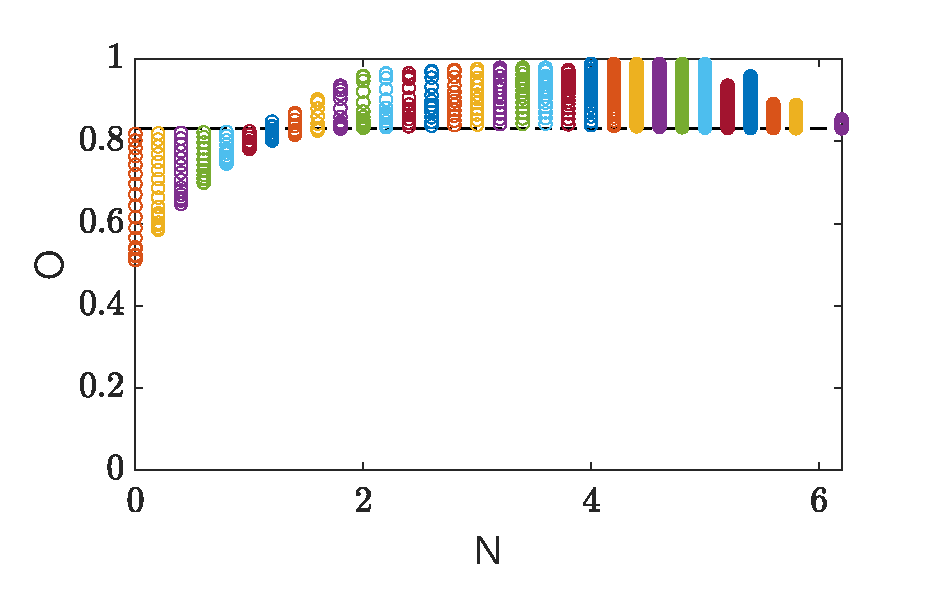
\includegraphics[width = 0.4\textwidth]{Figs/Fig4_clogging}
%    \caption{Phase transition at the power}
%    \label{fig:fig4-clogging}
%\end{figure}
%%%%%%%%%%%%%%%%%%%%%%%%%%%%%%%%%%%%%%%%%%%%%%
% \section{Clogging Dynamics}
%%%%%%%%%%%%%%%%%%%%%%%%%%%%%%%%%%%%%%%%%%%%%%%%5 
%
\textit{Clogging Dynamics}-- Besides erosion, another change in the network is the deposition/sedimentation of material on the boundary walls of the porous material. We name this dynamical change a ``clogging'' process as opposed to erosion. Contrary to erosion, the clogging behavior may cause some edges to block which effectively alters the network of connectivity and network behavior. This change in the connection between nodes through edges getting blocked can drastically alter porous structure behavior, e.g., causes a huge difference between effective and true porosity \cite{shima2021}. Despite the drastic change of network with blockages, we can still focus on the \textit{initial} change in the order parameter. The derivative of order parameter can be written as 
%
\begin{align}
    \frac{d\mathcal{O}}{dt} = \sum_{ij} \sum_{kl} \frac{\partial \mathcal{O}}{\partial q_{ij}} \frac{\partial q_{ij}}{\partial C_{kl}}  \frac{\partial C_{kl}}{\partial t} \label{eq:order-derivative}
\end{align}
%
where the last term changes sign from erosion to clogging, i.e., $\partial C_{kl}/\partial t = \pm \alpha \pi q_{kl} /r_{kl}^{n-3}\mu l_{kl}$ for erosion and clogging respectively. As a result, the magnitude of change in the order parameter equals that of erosion. Note that in Eq. \eqref{eq:order-derivative}, the second term depends on the network topology, and pore throat clogging results in the change of network topology at later times.
% The pore throat blockages results in the divergent of clogging results from just the negative of erosion. 
In short times, however, similar to the erosion, a phase transition exists at $n=3$. When  $n<3$ the network moves toward homogenization during the clogging process and when $n>3$ the flow moves toward the development of channeling instability. At later times, this initial trend, however, might not hold true due to the aforementioned complex changes in the connectivity network during the clogging process. 

%%%%%%%%%%%%%%%%%%%%%%%%%%%%%%%%%%%%%%%%%%%%%%%% 
% \section{Conclusion}
%%%%%%%%%%%%%%%%%%%%%%%%%%%%%%%%%%%%%%%%%%%%%%%
%
\textit{Conclusion}-- In summary, we analyzed the dynamics of the porous networks during erosion. We showed that depending on different erosion laws various network behaviors are observable. We used simple erosion laws, inspired by previously proposed models, and showed that depending on the rate of erosion the network can either move toward homogenization or toward developing a channeling instability. Next, we propose an order parameter to capture the phase transition behavior, and using a simplified model of two tubes we elucidated the physical origin of the phase transition behavior. 
In the case of clogging, since the network connectivity can vary significantly our approach does not hold at large times, however, the initial variation can be captured using our model where the results similarly show a behavior change at $n=3$. Our results signify the importance of local dynamics and feedback mechanism in long-time global behavior and complement similar feedback-induced studies for active conducting mediums~\cite{ocko2015feedback}. 

% \add{phase transition from channeling to full blocking in active porous structures \cite{ocko2015feedback}}

\textit{Acknowledgments}-- We would like to acknowledge Kavli Institute for the fruitful discussions and also MRSEC  DMR-2011754 and DMR-1420570 for the support. 

% \begin{figure}[h]
    % \centering
%     \includegraphics[width = 0.48\textwidth]{Figs/Fig2p_clogging.png}
%    \caption{Clogging in a network of pipes. The initial condition is shown with the label $t=0$ in the first row. Each row afterward corresponds to the simulation result after $N$ steps such that $\langle R_{t=N}\rangle=0.5 R_0$ where $R_0 = \langle R_{t=0}\rangle$; in other words the same amount of material is eroded in all cases. The erosion laws used here is $dR/dt = \alpha Q/R^n$ where $n$ varies for each row. The constant $\alpha$ in all cases are $1$ and time step $dt$ is chosen such that the maximum amount of increase in $R$ at each step is smaller than $0.01 R_0$. }\label{fig:fig2}
% \end{figure}


% \begin{itemize}
%    \item second order phase transition
%     \item intro
%    \item fig 4 for random network
%    \item clogging? 
% \end{itemize}











\bibliography{ref.bib}

\appendix





\end{document}
